% Options for packages loaded elsewhere
\PassOptionsToPackage{unicode}{hyperref}
\PassOptionsToPackage{hyphens}{url}
%
\documentclass[
]{book}
\title{My First Steps in Neuronal Networks}
\author{Axel Roth}
\date{2021-11-06}

\usepackage{amsmath,amssymb}
\usepackage{lmodern}
\usepackage{iftex}
\ifPDFTeX
  \usepackage[T1]{fontenc}
  \usepackage[utf8]{inputenc}
  \usepackage{textcomp} % provide euro and other symbols
\else % if luatex or xetex
  \usepackage{unicode-math}
  \defaultfontfeatures{Scale=MatchLowercase}
  \defaultfontfeatures[\rmfamily]{Ligatures=TeX,Scale=1}
\fi
% Use upquote if available, for straight quotes in verbatim environments
\IfFileExists{upquote.sty}{\usepackage{upquote}}{}
\IfFileExists{microtype.sty}{% use microtype if available
  \usepackage[]{microtype}
  \UseMicrotypeSet[protrusion]{basicmath} % disable protrusion for tt fonts
}{}
\makeatletter
\@ifundefined{KOMAClassName}{% if non-KOMA class
  \IfFileExists{parskip.sty}{%
    \usepackage{parskip}
  }{% else
    \setlength{\parindent}{0pt}
    \setlength{\parskip}{6pt plus 2pt minus 1pt}}
}{% if KOMA class
  \KOMAoptions{parskip=half}}
\makeatother
\usepackage{xcolor}
\IfFileExists{xurl.sty}{\usepackage{xurl}}{} % add URL line breaks if available
\IfFileExists{bookmark.sty}{\usepackage{bookmark}}{\usepackage{hyperref}}
\hypersetup{
  pdftitle={My First Steps in Neuronal Networks},
  pdfauthor={Axel Roth},
  hidelinks,
  pdfcreator={LaTeX via pandoc}}
\urlstyle{same} % disable monospaced font for URLs
\usepackage{color}
\usepackage{fancyvrb}
\newcommand{\VerbBar}{|}
\newcommand{\VERB}{\Verb[commandchars=\\\{\}]}
\DefineVerbatimEnvironment{Highlighting}{Verbatim}{commandchars=\\\{\}}
% Add ',fontsize=\small' for more characters per line
\usepackage{framed}
\definecolor{shadecolor}{RGB}{248,248,248}
\newenvironment{Shaded}{\begin{snugshade}}{\end{snugshade}}
\newcommand{\AlertTok}[1]{\textcolor[rgb]{0.94,0.16,0.16}{#1}}
\newcommand{\AnnotationTok}[1]{\textcolor[rgb]{0.56,0.35,0.01}{\textbf{\textit{#1}}}}
\newcommand{\AttributeTok}[1]{\textcolor[rgb]{0.77,0.63,0.00}{#1}}
\newcommand{\BaseNTok}[1]{\textcolor[rgb]{0.00,0.00,0.81}{#1}}
\newcommand{\BuiltInTok}[1]{#1}
\newcommand{\CharTok}[1]{\textcolor[rgb]{0.31,0.60,0.02}{#1}}
\newcommand{\CommentTok}[1]{\textcolor[rgb]{0.56,0.35,0.01}{\textit{#1}}}
\newcommand{\CommentVarTok}[1]{\textcolor[rgb]{0.56,0.35,0.01}{\textbf{\textit{#1}}}}
\newcommand{\ConstantTok}[1]{\textcolor[rgb]{0.00,0.00,0.00}{#1}}
\newcommand{\ControlFlowTok}[1]{\textcolor[rgb]{0.13,0.29,0.53}{\textbf{#1}}}
\newcommand{\DataTypeTok}[1]{\textcolor[rgb]{0.13,0.29,0.53}{#1}}
\newcommand{\DecValTok}[1]{\textcolor[rgb]{0.00,0.00,0.81}{#1}}
\newcommand{\DocumentationTok}[1]{\textcolor[rgb]{0.56,0.35,0.01}{\textbf{\textit{#1}}}}
\newcommand{\ErrorTok}[1]{\textcolor[rgb]{0.64,0.00,0.00}{\textbf{#1}}}
\newcommand{\ExtensionTok}[1]{#1}
\newcommand{\FloatTok}[1]{\textcolor[rgb]{0.00,0.00,0.81}{#1}}
\newcommand{\FunctionTok}[1]{\textcolor[rgb]{0.00,0.00,0.00}{#1}}
\newcommand{\ImportTok}[1]{#1}
\newcommand{\InformationTok}[1]{\textcolor[rgb]{0.56,0.35,0.01}{\textbf{\textit{#1}}}}
\newcommand{\KeywordTok}[1]{\textcolor[rgb]{0.13,0.29,0.53}{\textbf{#1}}}
\newcommand{\NormalTok}[1]{#1}
\newcommand{\OperatorTok}[1]{\textcolor[rgb]{0.81,0.36,0.00}{\textbf{#1}}}
\newcommand{\OtherTok}[1]{\textcolor[rgb]{0.56,0.35,0.01}{#1}}
\newcommand{\PreprocessorTok}[1]{\textcolor[rgb]{0.56,0.35,0.01}{\textit{#1}}}
\newcommand{\RegionMarkerTok}[1]{#1}
\newcommand{\SpecialCharTok}[1]{\textcolor[rgb]{0.00,0.00,0.00}{#1}}
\newcommand{\SpecialStringTok}[1]{\textcolor[rgb]{0.31,0.60,0.02}{#1}}
\newcommand{\StringTok}[1]{\textcolor[rgb]{0.31,0.60,0.02}{#1}}
\newcommand{\VariableTok}[1]{\textcolor[rgb]{0.00,0.00,0.00}{#1}}
\newcommand{\VerbatimStringTok}[1]{\textcolor[rgb]{0.31,0.60,0.02}{#1}}
\newcommand{\WarningTok}[1]{\textcolor[rgb]{0.56,0.35,0.01}{\textbf{\textit{#1}}}}
\usepackage{longtable,booktabs,array}
\usepackage{calc} % for calculating minipage widths
% Correct order of tables after \paragraph or \subparagraph
\usepackage{etoolbox}
\makeatletter
\patchcmd\longtable{\par}{\if@noskipsec\mbox{}\fi\par}{}{}
\makeatother
% Allow footnotes in longtable head/foot
\IfFileExists{footnotehyper.sty}{\usepackage{footnotehyper}}{\usepackage{footnote}}
\makesavenoteenv{longtable}
\usepackage{graphicx}
\makeatletter
\def\maxwidth{\ifdim\Gin@nat@width>\linewidth\linewidth\else\Gin@nat@width\fi}
\def\maxheight{\ifdim\Gin@nat@height>\textheight\textheight\else\Gin@nat@height\fi}
\makeatother
% Scale images if necessary, so that they will not overflow the page
% margins by default, and it is still possible to overwrite the defaults
% using explicit options in \includegraphics[width, height, ...]{}
\setkeys{Gin}{width=\maxwidth,height=\maxheight,keepaspectratio}
% Set default figure placement to htbp
\makeatletter
\def\fps@figure{htbp}
\makeatother
\setlength{\emergencystretch}{3em} % prevent overfull lines
\providecommand{\tightlist}{%
  \setlength{\itemsep}{0pt}\setlength{\parskip}{0pt}}
\setcounter{secnumdepth}{5}
\usepackage{booktabs}
\usepackage{amsthm}
\makeatletter
\def\thm@space@setup{%
  \thm@preskip=8pt plus 2pt minus 4pt
  \thm@postskip=\thm@preskip
}
\makeatother
\ifLuaTeX
  \usepackage{selnolig}  % disable illegal ligatures
\fi
\usepackage[]{natbib}
\bibliographystyle{apalike}

\begin{document}
\maketitle

{
\setcounter{tocdepth}{1}
\tableofcontents
}
\hypertarget{about}{%
\chapter{About}\label{about}}

\hypertarget{me}{%
\section{Me}\label{me}}

Hello, my name is Axel Roth and at the moment im studieing math at a master degree. In the same moment im working half-time in the finance field and programming in a wide range of tasks like index replication, factormodels, data visualisation, datamanagement, shiny applications, documantations with rmarkdown, building internal packages and much more. So the most of my experiece i gained was around R and all its features. And now the iterresting question\ldots{} Why do i want to write a beginners guide in the field of Neuronal Networks?\\
Its simple, at the moment i have a lecture in that we learn how to programm a Neuronal Network from scratch with basic packages from python and i want to share my experience. Additionaly i learned all i know from free sources of the internet and thats why i want to give something back. Furthermore its a good use-case to write my first things in english and test the fancy Bookdown and GitBook features.

\hypertarget{the-book}{%
\section{The Book}\label{the-book}}

This Book will be more or the less the documentation of my lecture ``Finance Project'' in that we learn to programm a simple Perceptron (the simplest Neuronal Network) and then we will continue with a multi layer perceptron and finish with a slight insight into decision trees. On this journey, we will test the Neuronal Network in different examples that are easy to reproduce. Because these are my first steps in this field, i need to appolagice for my terrible spelling and cant guarantee you the best quality, but maybe this is the best way to educate and attract unexperienced readers to have a look into this field.

\hypertarget{how-it-works}{%
\section{How it works}\label{how-it-works}}

Im coding this book in the IDE R-Studio with the framework of Bookdown and embed python code that is made possible by the reticulate package. Thats why i need to load the python interpreter in the following R-chunk:

\begin{Shaded}
\begin{Highlighting}[]
\FunctionTok{library}\NormalTok{(reticulate)}
\FunctionTok{Sys.setenv}\NormalTok{(}\AttributeTok{RETICULATE\_PYTHON =} \StringTok{"D:}\SpecialCharTok{\textbackslash{}\textbackslash{}}\StringTok{WinPython2}\SpecialCharTok{\textbackslash{}\textbackslash{}}\StringTok{WPy64{-}3950}\SpecialCharTok{\textbackslash{}\textbackslash{}}\StringTok{python{-}3.9.5.amd64}\SpecialCharTok{\textbackslash{}\textbackslash{}}\StringTok{"}\NormalTok{)}
\end{Highlighting}
\end{Shaded}

Additionaly im using a fully portable version of R-Studio, R and python. Its nice to have if you want to switch for example between university PCs and your own. R-Studio supports it and python can be downloaded via WinPython to be fully portable.

\hypertarget{a-single-perceptron}{%
\chapter{A single Perceptron}\label{a-single-perceptron}}

In this chapter i will teach you how to code a single Perceptron in Python with more or the less only the numpy package. Numpy uses a vectorizible math structure in which you can easily calculate elementwise or do stuff like normal matrix multiplications with just a symbol (i always interprete Vectors as one dimensional matrixes!). At the most of the times its just translating math formulars into python code without changing its structure.\\
First of all we are starting with the needed parameters, that are explained later:

Number of runs over the training data := \texttt{train\_n}\\
Learning rate := \(\alpha =\) \texttt{alpha}\\
and the activation function:\\
\[ 
step(s)= 
\begin{cases}
    1,& s   \geq 0\\
    0,& s < 0
\end{cases}
\]
This function is named the heavyside-function and should be the easiest activation function to start with.

The traings dataset is the following:
\[
\left[
\begin{array}{cc|c}
x_i,_1 & x_i,_2 & y_i \\
\end{array}
\right]
\]
\[
\left[
\begin{array}{cc|c}
0 & 0 & 0 \\
0 & 1 & 1 \\
1 & 0 & 1 \\
1 & 1 & 1 \\
\end{array}
\right]
\]
The provided traings dataset contains the \texttt{X\_train} matrix with two inputs each scenario and the \texttt{Y\_train} matrix with the correct output. If your looking exactly you can see that this is the OR-Gate. Later you will see why these type of problems are the only suitable things to do with a single neuron.\\
For a wider use we will now change the \texttt{X\_train} matrix a little bit by adding a column with ones on the left side of it. Now you will not understand but later you will. In short, its a dummy value to make it possible to shift the NN, so it can be better fitted. The new traings dataset looks like this:
\[
\left[
\begin{array}{ccc|c}
x_i,_0 & x_i,_1 & x_i,_2 & y_i \\
\end{array}
\right]
\]
\[
\left[
\begin{array}{ccc|c}
1 & 0 & 0 & 0 \\
1 & 0 & 1 & 1 \\
1 & 1 & 0 & 1 \\
1 & 1 & 1 & 1 \\
\end{array}
\right]
\]

The needed python imports and default options are the following:

\begin{Shaded}
\begin{Highlighting}[]
\ImportTok{import}\NormalTok{ numpy }\ImportTok{as}\NormalTok{ np}
\ImportTok{import}\NormalTok{ random }\ImportTok{as}\NormalTok{ ra}
\ImportTok{import}\NormalTok{ pandas }\ImportTok{as}\NormalTok{ pd}
\ImportTok{import}\NormalTok{ matplotlib.pyplot }\ImportTok{as}\NormalTok{ pyplot}
\NormalTok{pd.set\_option(}\StringTok{\textquotesingle{}display.max\_rows\textquotesingle{}}\NormalTok{, }\DecValTok{500}\NormalTok{)}
\NormalTok{pd.set\_option(}\StringTok{\textquotesingle{}display.max\_columns\textquotesingle{}}\NormalTok{, }\DecValTok{500}\NormalTok{)}
\NormalTok{pd.set\_option(}\StringTok{\textquotesingle{}display.width\textquotesingle{}}\NormalTok{, }\DecValTok{1000}\NormalTok{)}
\end{Highlighting}
\end{Shaded}

( Do you see more imports than only the numpy package? \href{https://www.youtube.com/watch?v=dQw4w9WgXcQ}{Yes} or No )

Now that we have all the needed parameters and settings, i can give you a quick overview of the algorithm.

\hypertarget{neural-network-basics}{%
\section{Neural Network Basics}\label{neural-network-basics}}

In a NN we are having two basic parts, the forward pass and backward pass. In the forward pass we are calculating the weighted sum of each input with its weights of the layer to get the output. In the backward pass we are analysing the error to adjust the weights accordingly. This is it! This is all a NN will do. Now that you know, see you. I explained everything to you. Have a good life\ldots{}\\
Ahh no no ok we have a look deeper into it :)

Whats exactly is the forward pass in a single Perceptron? Its just the weighted sum like i said, so you have with the dimensions included for one scenario out of the traingdata the folowing:
\[
  step(W^{(1,3)} \cdot x^{(3,1)}) = y^{(1,1)}
\]
That is the normal approach to iterate over all scenarios in the trainingdata\ldots{}\\
But i think its not the right way to describe it because it gets very confusing to interpret it for all scenarios.

My next approach is to consider all scenarios in the trainingdata in one formular. If your data isnt that huge, its a much faster approach aswell. First of all we need to interpret the new dimensions of \(W\) and \(X\).\\
We have \(X\) as:
\[
  X = \left[
  \begin{array}{ccc}
  1 & 0 & 0 \\
  1 & 0 & 1 \\
  1 & 1 & 0 \\
  1 & 1 & 1 \\
  \end{array}
  \right]
\]
each row describes the inputs for each neuron in the scenario \(i\).\\
For the weights \(W\) we have for example:
\[
  W =\left[
  \begin{array}{c}
  0.1 \\ 
  0.2 \\ 
  0.3 \\
  \end{array}
  \right]
\]
The new formular looks like this:
\[
  step(X \cdot W) = Y
\]
For example if you take a look at the \(i\)-th row or scenario of \(X\) you will see the following:
\[
  Y_i,_0 = step([X_i,_0 \cdot W_0,_0 + X_i,_1 \cdot W_1,_0 + X_i,_2 \cdot W_2,_0])
\]
and \(Y_i,_0\) is the approximated output of the \(i\)-th scenario. Now we can look at the NN and compare the formular with it:\\
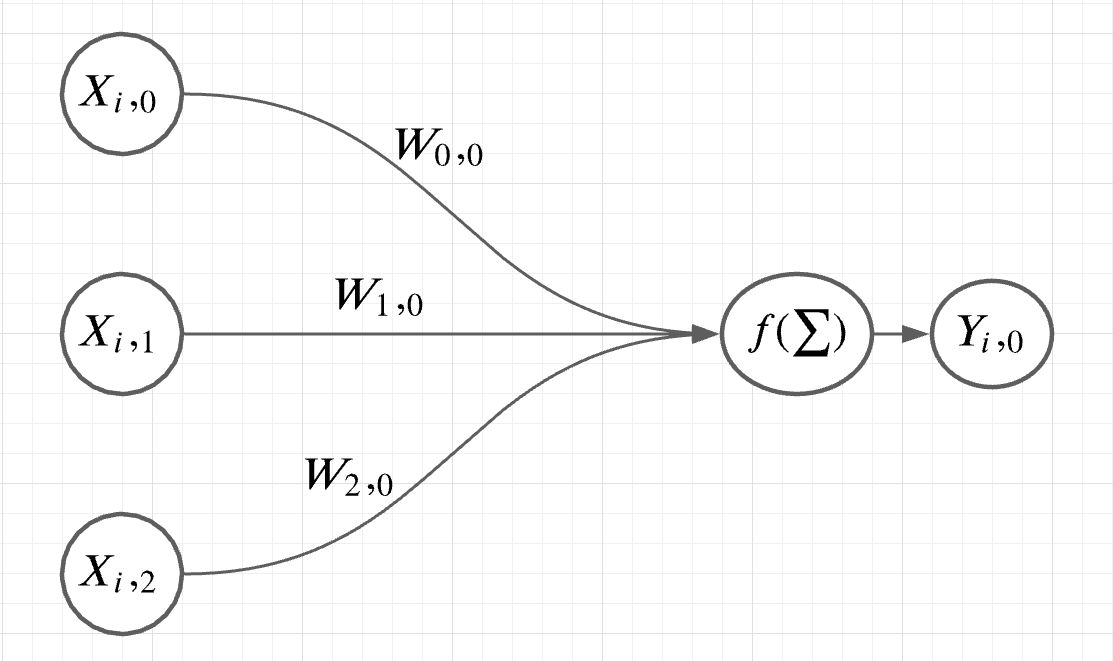
\includegraphics[width=0.5\textwidth,height=\textheight]{./img/NN_01_v2.png}
ZZYes it is the same, its the weighted sum of the inputs and evaluated with it the activationfunction to calculate the output of the scenario \(i\).

\hypertarget{forward-pass}{%
\section{Forward pass}\label{forward-pass}}

Now we create the so called \texttt{forward()} function in python:

\begin{Shaded}
\begin{Highlighting}[]
\KeywordTok{def}\NormalTok{ forward(X, W):}
  \ControlFlowTok{return}\NormalTok{( step(X }\OperatorTok{@}\NormalTok{ W) )}
\end{Highlighting}
\end{Shaded}

(Numpy provides us with the \texttt{@} symbol to make a matrix multiplication and the \texttt{.T} to transpose)

Because we want to put one dimensional matrixes into the \texttt{step()} function we need to use numpy for the if-else statement:

\begin{Shaded}
\begin{Highlighting}[]
\KeywordTok{def}\NormalTok{ step(s):}
  \ControlFlowTok{return}\NormalTok{( np.where(s }\OperatorTok{\textgreater{}=} \DecValTok{0}\NormalTok{, }\DecValTok{1}\NormalTok{, }\DecValTok{0}\NormalTok{) )}
\end{Highlighting}
\end{Shaded}

Here an small example for the forward pass:

\begin{Shaded}
\begin{Highlighting}[]
\NormalTok{X }\OperatorTok{=}\NormalTok{ np.array([}
\NormalTok{  [}\DecValTok{1}\NormalTok{,}\DecValTok{0}\NormalTok{,}\DecValTok{0}\NormalTok{],}
\NormalTok{  [}\DecValTok{1}\NormalTok{,}\DecValTok{0}\NormalTok{,}\DecValTok{1}\NormalTok{],}
\NormalTok{  [}\DecValTok{1}\NormalTok{,}\DecValTok{1}\NormalTok{,}\DecValTok{0}\NormalTok{],}
\NormalTok{  [}\DecValTok{1}\NormalTok{,}\DecValTok{1}\NormalTok{,}\DecValTok{1}\NormalTok{],}
\NormalTok{])}
\NormalTok{W }\OperatorTok{=}\NormalTok{ np.array([}
\NormalTok{  [}\FloatTok{0.1}\NormalTok{], }
\NormalTok{  [}\FloatTok{0.2}\NormalTok{], }
\NormalTok{  [}\FloatTok{0.3}\NormalTok{]}
\NormalTok{])}
\NormalTok{Y\_approx }\OperatorTok{=}\NormalTok{ forward(X, W)}
\BuiltInTok{print}\NormalTok{(Y\_approx)}
\end{Highlighting}
\end{Shaded}

\begin{verbatim}
## [[1]
##  [1]
##  [1]
##  [1]]
\end{verbatim}

And these are all the generated outputs of our NN over all scenarios. Now we need to calculate the error and adjust the weights accordingly.

\hypertarget{backward-pass}{%
\section{backward pass}\label{backward-pass}}

To adjust the weights we need the Delta-Rule:
\[
  W(t+1) = W(t) + \Delta W(t)
\]
with
\[
  \Delta W(t) = \alpha \cdot X^{T} \cdot (Y - \hat{Y})
\]
and \(\hat{Y}\) is the output of the NN.

\begin{Shaded}
\begin{Highlighting}[]
\KeywordTok{def}\NormalTok{ backward(W, X, Y, alpha, Y\_approx):}
    \ControlFlowTok{return}\NormalTok{(W }\OperatorTok{+}\NormalTok{ alpha }\OperatorTok{*}\NormalTok{ X.T }\OperatorTok{@}\NormalTok{ (Y }\OperatorTok{{-}}\NormalTok{ Y\_approx))}
\end{Highlighting}
\end{Shaded}

with the result of the forward pass and example data we have the following:

\begin{Shaded}
\begin{Highlighting}[]
\NormalTok{Y }\OperatorTok{=}\NormalTok{ np.array([}
\NormalTok{  [}\DecValTok{0}\NormalTok{],}
\NormalTok{  [}\DecValTok{1}\NormalTok{],}
\NormalTok{  [}\DecValTok{1}\NormalTok{],}
\NormalTok{  [}\DecValTok{1}\NormalTok{]}
\NormalTok{])}
\NormalTok{alpha }\OperatorTok{=} \DecValTok{1}
\NormalTok{W }\OperatorTok{=}\NormalTok{ backward(W, X, Y, alpha, Y\_approx)}
\end{Highlighting}
\end{Shaded}

and this is the new weight.

\hypertarget{single-perceptron}{%
\section{Single Perceptron}\label{single-perceptron}}

Now we want to do the same process multiple times, to train the NN:

\begin{Shaded}
\begin{Highlighting}[]
\NormalTok{X }\OperatorTok{=}\NormalTok{ np.array([}
\NormalTok{  [}\DecValTok{1}\NormalTok{,}\DecValTok{0}\NormalTok{,}\DecValTok{0}\NormalTok{],}
\NormalTok{  [}\DecValTok{1}\NormalTok{,}\DecValTok{0}\NormalTok{,}\DecValTok{1}\NormalTok{],}
\NormalTok{  [}\DecValTok{1}\NormalTok{,}\DecValTok{1}\NormalTok{,}\DecValTok{0}\NormalTok{],}
\NormalTok{  [}\DecValTok{1}\NormalTok{,}\DecValTok{1}\NormalTok{,}\DecValTok{1}\NormalTok{],}
\NormalTok{])}
\NormalTok{Y }\OperatorTok{=}\NormalTok{ np.array([}
\NormalTok{  [}\DecValTok{0}\NormalTok{],}
\NormalTok{  [}\DecValTok{1}\NormalTok{],}
\NormalTok{  [}\DecValTok{1}\NormalTok{],}
\NormalTok{  [}\DecValTok{1}\NormalTok{]}
\NormalTok{])}
\NormalTok{W }\OperatorTok{=}\NormalTok{ np.array([}
\NormalTok{  [}\FloatTok{0.1}\NormalTok{], }
\NormalTok{  [}\FloatTok{0.2}\NormalTok{], }
\NormalTok{  [}\FloatTok{0.3}\NormalTok{]}
\NormalTok{])}
\NormalTok{alpha }\OperatorTok{=} \DecValTok{1}

\NormalTok{errors }\OperatorTok{=}\NormalTok{ []}
\ControlFlowTok{for}\NormalTok{ i }\KeywordTok{in} \BuiltInTok{range}\NormalTok{(}\DecValTok{20}\NormalTok{):}
\NormalTok{  Y\_approx }\OperatorTok{=}\NormalTok{ forward(X, W)}
\NormalTok{  errors.append(Y }\OperatorTok{{-}}\NormalTok{ Y\_approx)}
\NormalTok{  W }\OperatorTok{=}\NormalTok{ backward(W, X, Y, alpha, Y\_approx)}
\end{Highlighting}
\end{Shaded}

The KNN is trained now. Now we want to look at the error. We want to measure the mean-square-error with the following formula:
\[
  Error_i = \frac{1}{2} \cdot \sum(Y-\hat{Y})^2
\]
or as python code:

\begin{Shaded}
\begin{Highlighting}[]
\KeywordTok{def}\NormalTok{ mean\_square\_error(error):}
  \ControlFlowTok{return}\NormalTok{( }\FloatTok{0.5} \OperatorTok{*}\NormalTok{ np.}\BuiltInTok{sum}\NormalTok{(error }\OperatorTok{**} \DecValTok{2}\NormalTok{) )}
\end{Highlighting}
\end{Shaded}

Now we need to calculate the mean-square-error for each element in the list \texttt{errors} which is made with \texttt{map}:

\begin{Shaded}
\begin{Highlighting}[]
\NormalTok{mean\_square\_errors }\OperatorTok{=}\NormalTok{ np.array(}\BuiltInTok{list}\NormalTok{(}\BuiltInTok{map}\NormalTok{(mean\_square\_error, errors)))}
\end{Highlighting}
\end{Shaded}

To plot, im using the following function:

\begin{Shaded}
\begin{Highlighting}[]
\KeywordTok{def}\NormalTok{ plot\_error(errors, title):}
\NormalTok{  x }\OperatorTok{=} \BuiltInTok{list}\NormalTok{(}\BuiltInTok{range}\NormalTok{(}\BuiltInTok{len}\NormalTok{(errors)))}
\NormalTok{  y }\OperatorTok{=}\NormalTok{ np.array(errors)}
\NormalTok{  pyplot.figure(figsize}\OperatorTok{=}\NormalTok{(}\DecValTok{6}\NormalTok{,}\DecValTok{6}\NormalTok{))}
\NormalTok{  pyplot.plot(x, y, }\StringTok{"g"}\NormalTok{, linewidth}\OperatorTok{=}\DecValTok{1}\NormalTok{)}
\NormalTok{  pyplot.xlabel(}\StringTok{"Iterations"}\NormalTok{, fontsize }\OperatorTok{=} \DecValTok{16}\NormalTok{)}
\NormalTok{  pyplot.ylabel(}\StringTok{"Mean Square Error"}\NormalTok{, fontsize }\OperatorTok{=} \DecValTok{16}\NormalTok{)}
\NormalTok{  pyplot.title(title)}
\NormalTok{  pyplot.ylim(}\OperatorTok{{-}}\FloatTok{0.01}\NormalTok{,}\BuiltInTok{max}\NormalTok{(errors)}\OperatorTok{*}\FloatTok{1.2}\NormalTok{)}
\NormalTok{  pyplot.show()}
  
  
\NormalTok{plot\_error(mean\_square\_errors, }\StringTok{"Mean{-}Square{-}Errors of a single Perceptron"}\NormalTok{)}
\end{Highlighting}
\end{Shaded}

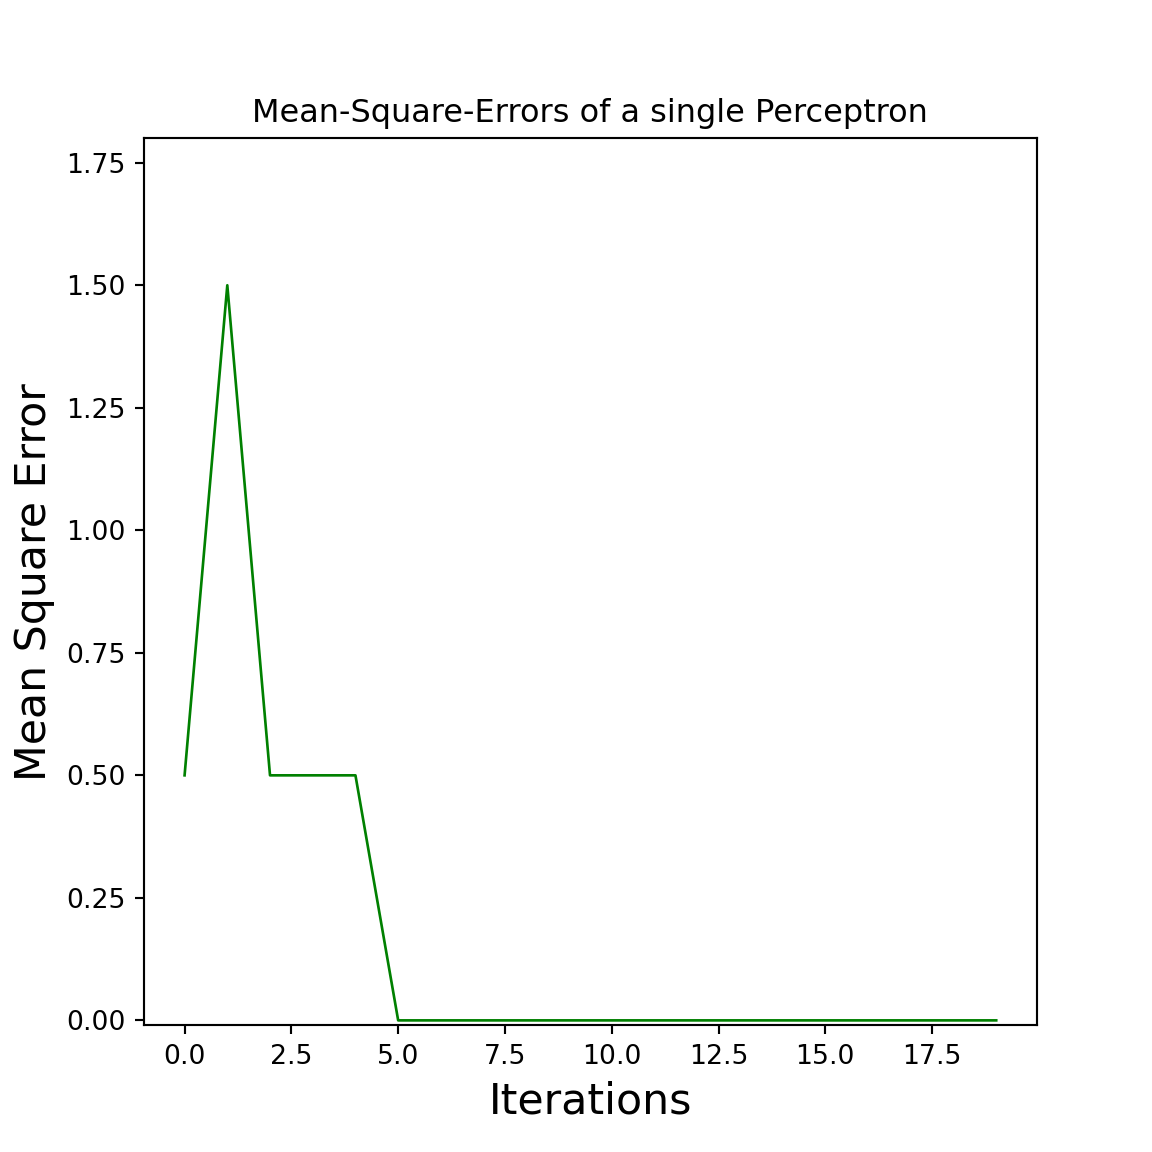
\includegraphics{gitbook-demo_files/figure-latex/unnamed-chunk-11-1.pdf}

If you survived until now, you have learned how you can programm a single Perceptron!

\hypertarget{appendix-full-code}{%
\section{Appendix (full code)}\label{appendix-full-code}}

\begin{Shaded}
\begin{Highlighting}[]
\ImportTok{import}\NormalTok{ numpy }\ImportTok{as}\NormalTok{ np}
\ImportTok{import}\NormalTok{ random }\ImportTok{as}\NormalTok{ ra}
\ImportTok{import}\NormalTok{ pandas }\ImportTok{as}\NormalTok{ pd}
\ImportTok{import}\NormalTok{ matplotlib.pyplot }\ImportTok{as}\NormalTok{ pyplot}
\NormalTok{pd.set\_option(}\StringTok{\textquotesingle{}display.max\_rows\textquotesingle{}}\NormalTok{, }\DecValTok{500}\NormalTok{)}
\NormalTok{pd.set\_option(}\StringTok{\textquotesingle{}display.max\_columns\textquotesingle{}}\NormalTok{, }\DecValTok{500}\NormalTok{)}
\NormalTok{pd.set\_option(}\StringTok{\textquotesingle{}display.width\textquotesingle{}}\NormalTok{, }\DecValTok{1000}\NormalTok{)}

\NormalTok{X }\OperatorTok{=}\NormalTok{ np.array([}
\NormalTok{  [}\DecValTok{1}\NormalTok{,}\DecValTok{0}\NormalTok{,}\DecValTok{0}\NormalTok{],}
\NormalTok{  [}\DecValTok{1}\NormalTok{,}\DecValTok{0}\NormalTok{,}\DecValTok{1}\NormalTok{],}
\NormalTok{  [}\DecValTok{1}\NormalTok{,}\DecValTok{1}\NormalTok{,}\DecValTok{0}\NormalTok{],}
\NormalTok{  [}\DecValTok{1}\NormalTok{,}\DecValTok{1}\NormalTok{,}\DecValTok{1}\NormalTok{],}
\NormalTok{])}
\NormalTok{Y }\OperatorTok{=}\NormalTok{ np.array([}
\NormalTok{  [}\DecValTok{0}\NormalTok{],}
\NormalTok{  [}\DecValTok{1}\NormalTok{],}
\NormalTok{  [}\DecValTok{1}\NormalTok{],}
\NormalTok{  [}\DecValTok{1}\NormalTok{]}
\NormalTok{])}
\NormalTok{W }\OperatorTok{=}\NormalTok{ np.array([}
\NormalTok{  [}\FloatTok{0.1}\NormalTok{], }
\NormalTok{  [}\FloatTok{0.2}\NormalTok{], }
\NormalTok{  [}\FloatTok{0.3}\NormalTok{]}
\NormalTok{])}
\NormalTok{alpha }\OperatorTok{=} \DecValTok{1}


\KeywordTok{def}\NormalTok{ step(s):}
  \ControlFlowTok{return}\NormalTok{( np.where(s }\OperatorTok{\textgreater{}=} \DecValTok{0}\NormalTok{, }\DecValTok{1}\NormalTok{, }\DecValTok{0}\NormalTok{) )}


\KeywordTok{def}\NormalTok{ forward(X, W):}
  \ControlFlowTok{return}\NormalTok{( step(X }\OperatorTok{@}\NormalTok{ W) )}

\KeywordTok{def}\NormalTok{ backward(W, X, Y, alpha, Y\_approx):}
    \ControlFlowTok{return}\NormalTok{(W }\OperatorTok{+}\NormalTok{ alpha }\OperatorTok{*}\NormalTok{ X.T }\OperatorTok{@}\NormalTok{ (Y }\OperatorTok{{-}}\NormalTok{ Y\_approx))}
  
  
\NormalTok{errors }\OperatorTok{=}\NormalTok{ []}
\ControlFlowTok{for}\NormalTok{ i }\KeywordTok{in} \BuiltInTok{range}\NormalTok{(}\DecValTok{20}\NormalTok{):}
\NormalTok{  Y\_approx }\OperatorTok{=}\NormalTok{ forward(X, W)}
\NormalTok{  errors.append(Y }\OperatorTok{{-}}\NormalTok{ Y\_approx)}
\NormalTok{  W }\OperatorTok{=}\NormalTok{ backward(W, X, Y, alpha, Y\_approx)}
  
  
  
\KeywordTok{def}\NormalTok{ mean\_square\_error(error):}
  \ControlFlowTok{return}\NormalTok{( }\FloatTok{0.5} \OperatorTok{*}\NormalTok{ np.}\BuiltInTok{sum}\NormalTok{(error }\OperatorTok{**} \DecValTok{2}\NormalTok{) )}


\NormalTok{mean\_square\_errors }\OperatorTok{=}\NormalTok{ np.array(}\BuiltInTok{list}\NormalTok{(}\BuiltInTok{map}\NormalTok{(mean\_square\_error, errors)))}


\KeywordTok{def}\NormalTok{ plot\_error(errors, title):}
\NormalTok{  x }\OperatorTok{=} \BuiltInTok{list}\NormalTok{(}\BuiltInTok{range}\NormalTok{(}\BuiltInTok{len}\NormalTok{(errors)))}
\NormalTok{  y }\OperatorTok{=}\NormalTok{ np.array(errors)}
\NormalTok{  pyplot.figure(figsize}\OperatorTok{=}\NormalTok{(}\DecValTok{6}\NormalTok{,}\DecValTok{6}\NormalTok{))}
\NormalTok{  pyplot.plot(x, y, }\StringTok{"g"}\NormalTok{, linewidth}\OperatorTok{=}\DecValTok{1}\NormalTok{)}
\NormalTok{  pyplot.xlabel(}\StringTok{"Iterations"}\NormalTok{, fontsize }\OperatorTok{=} \DecValTok{16}\NormalTok{)}
\NormalTok{  pyplot.ylabel(}\StringTok{"Mean Square Error"}\NormalTok{, fontsize }\OperatorTok{=} \DecValTok{16}\NormalTok{)}
\NormalTok{  pyplot.title(title)}
\NormalTok{  pyplot.ylim(}\OperatorTok{{-}}\FloatTok{0.01}\NormalTok{,}\BuiltInTok{max}\NormalTok{(errors)}\OperatorTok{*}\FloatTok{1.2}\NormalTok{)}
\NormalTok{  pyplot.xticks(x)}
\NormalTok{  pyplot.show()}
  
  
\NormalTok{plot\_error(mean\_square\_errors, }\StringTok{"Mean{-}Square{-}Errors of a single Perceptron"}\NormalTok{)}
\end{Highlighting}
\end{Shaded}


  \bibliography{book.bib,packages.bib}

\end{document}
